\documentclass{article}
\usepackage[utf8]{inputenc}
\usepackage[spanish]{babel}
\usepackage{listings}
\usepackage{graphicx}
\graphicspath{ {images/} }
\usepackage{cite}

\begin{document}

\begin{titlepage}
    \begin{center}
        \vspace*{1cm}
            
        \Huge
        \textbf{Videojuego}
            
        \vspace{0.5cm}
        \LARGE
        Informática II
            
            
        \vspace{1.5cm}
        
        \textbf{Marcela Flórez Orellano} 
        
        \vspace{0.3cm}
        \LARGE
        
        \textbf{Ferney Mejía Pérez}
            
        \vfill
            
        \vspace{0.8cm}
            
        \Large
        Departamento de Ingeniería Electrónica y Telecomunicaciones\\
        Universidad de Antioquia\\
        Medellín-Antioquia\\
        Octubre de 2021
         
            
    \end{center}
\end{titlepage}


\tableofcontents
\newpage


\section{Sección introductoria}\label{intro}
El presente proyecto hace énfasis en la implementación de las ideas principales del proyecto final correspondiente al curso en proceso, informática II, la cual tiene un enfoque de enseñanza en el lenguaje de programación C++, de tal motivo que, se realizarán diversos ejercicios de aprendizaje con el fin de adquirir lógica computacional y la habilidad necesaria para la solución de problemas comunes en la programación. Por lo tanto, para este proyecto se tiene de inicio la creación del esquema organizacional del cual se desprenderán las diferentes ideas que componen el cuerpo del juego correspondiente al mencionado proyecto.

Ahora bien, con respecto al juego, se tiene una idea global del mismo, en la cual se puede competir en diferentes galaxias para ser el mejor piloto intergaláctico del universo conocible. Se cuenta con diversos mapas en los que los contenidos galácticos cambian, igual que los competidores.  

\section{Sección de contenido} \label{contenido}
A continuación se presentan las ideas pertenecientes al esquema organizacional del juego:

\subsection{Esquema de las clases a implementar }

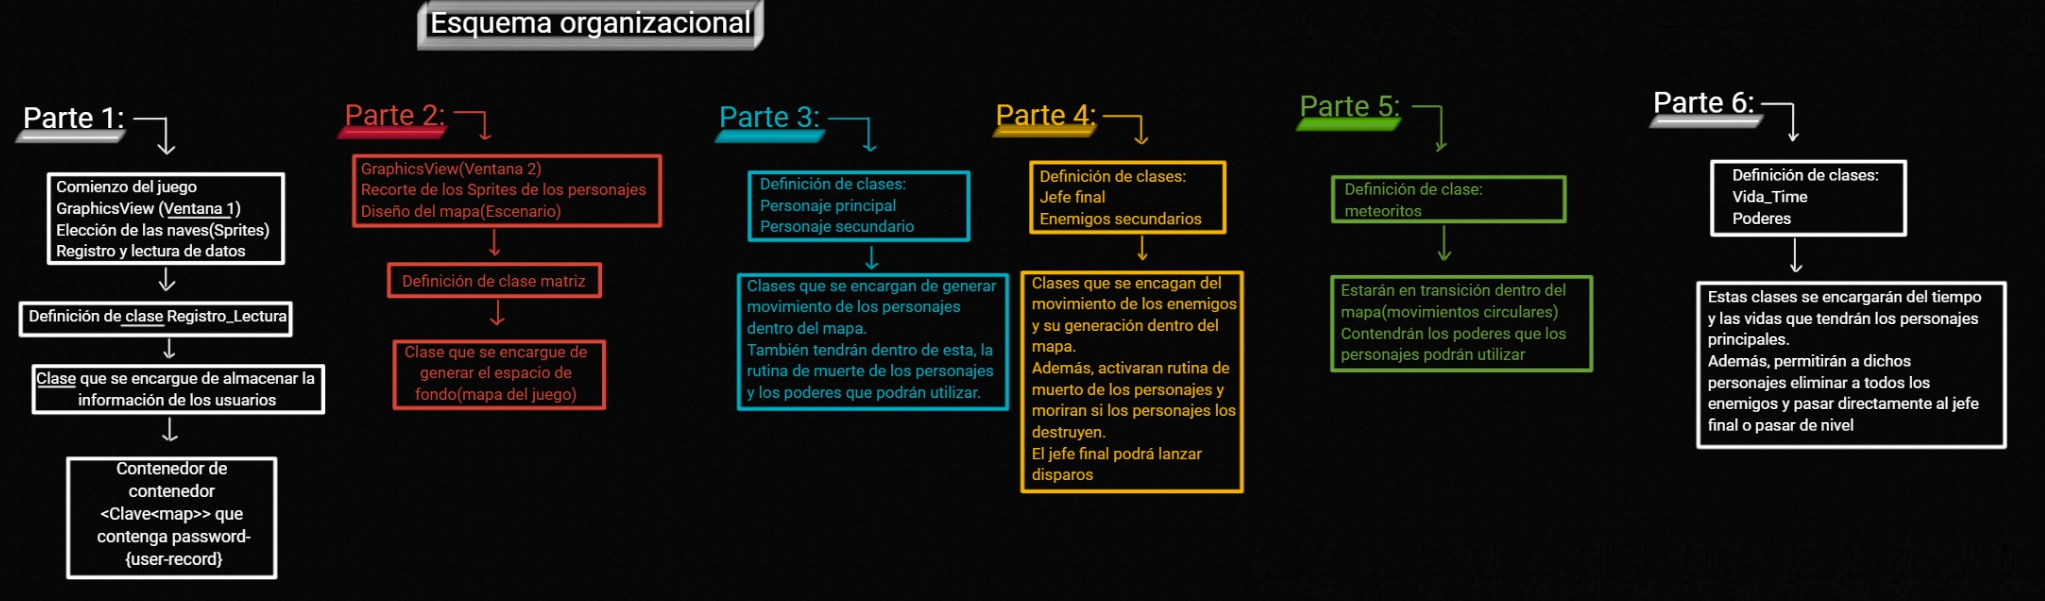
\includegraphics[scale=0.59]{Ideación/Images/esquema-clases.jpeg}


\subsection{Entorno}
El juego tendrá un entorno desarrollado en el espacio sideral, en el cual habrá múltiples galaxias a las cuales acceder para realizar competiciones en un mínimo de tiempo de tres minutos por nivel. 

En la introducción del juego se podrá presenciar el nombre del videojuego y el botón de inicio:


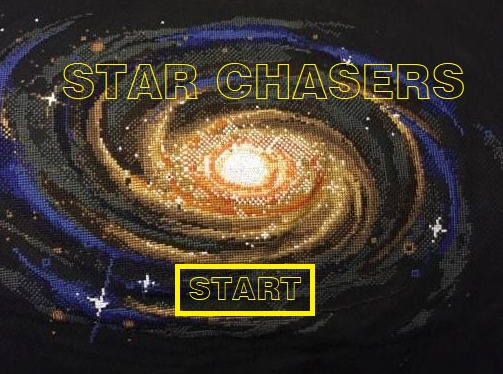
\includegraphics[scale=0.59]{Ideación/Images/Start.jpeg}


En general se podrá presenciar en la parte superior del mapa el tiempo, el nivel y el número de vidas que posee el jugador. 

EL fondo para el nivel 1: 

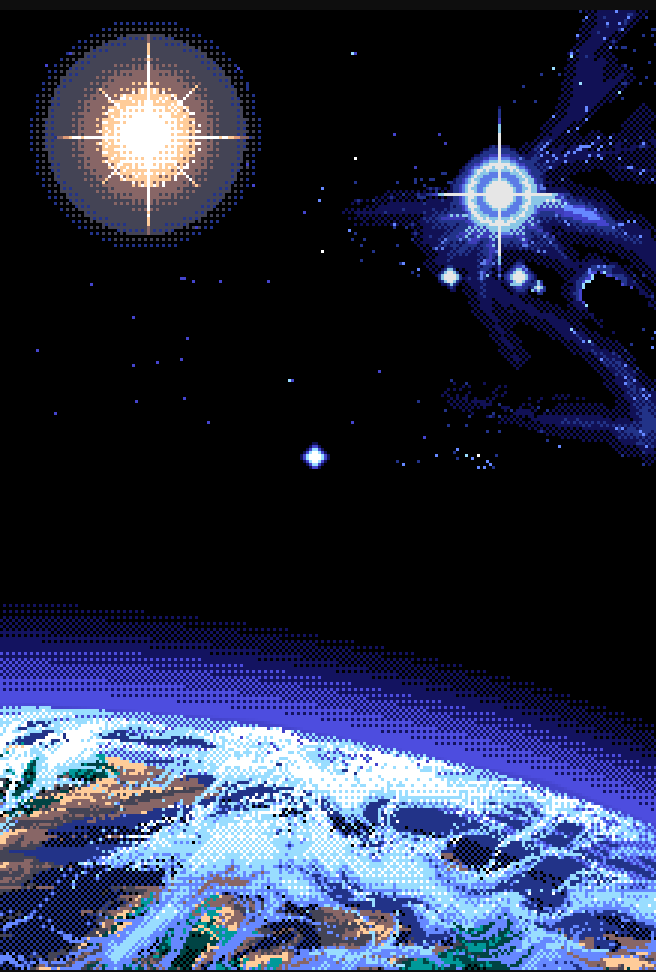
\includegraphics[scale=0.40]{Ideación/Images/mapa1.png}

El fondo para el nivel 2:

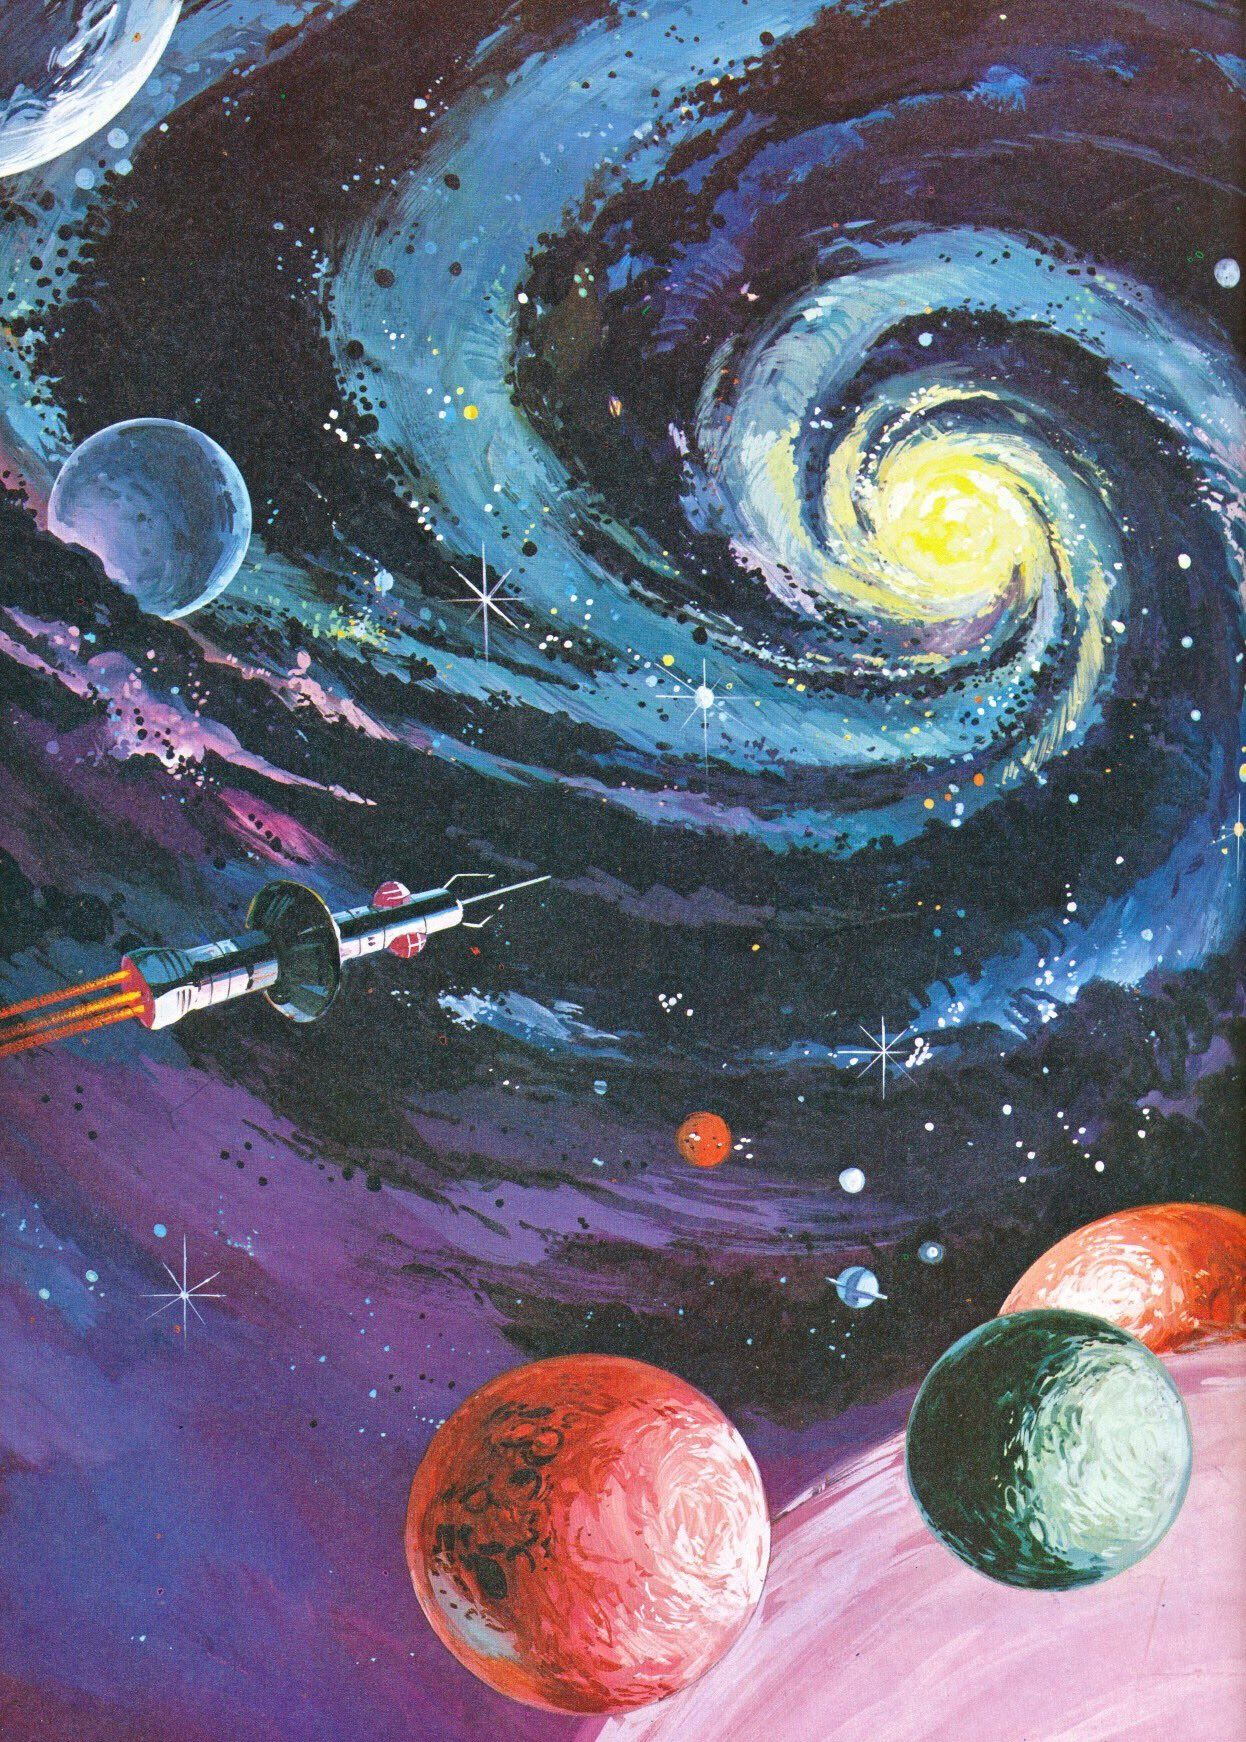
\includegraphics[scale=0.21]{Ideación/Images/mapa2.jpeg}

Además, la visualización del personaje moviéndose en el mapa será de manera vertical y horizontal, describiendo el tipo de movimiento presentado en la siguiente imagen:  

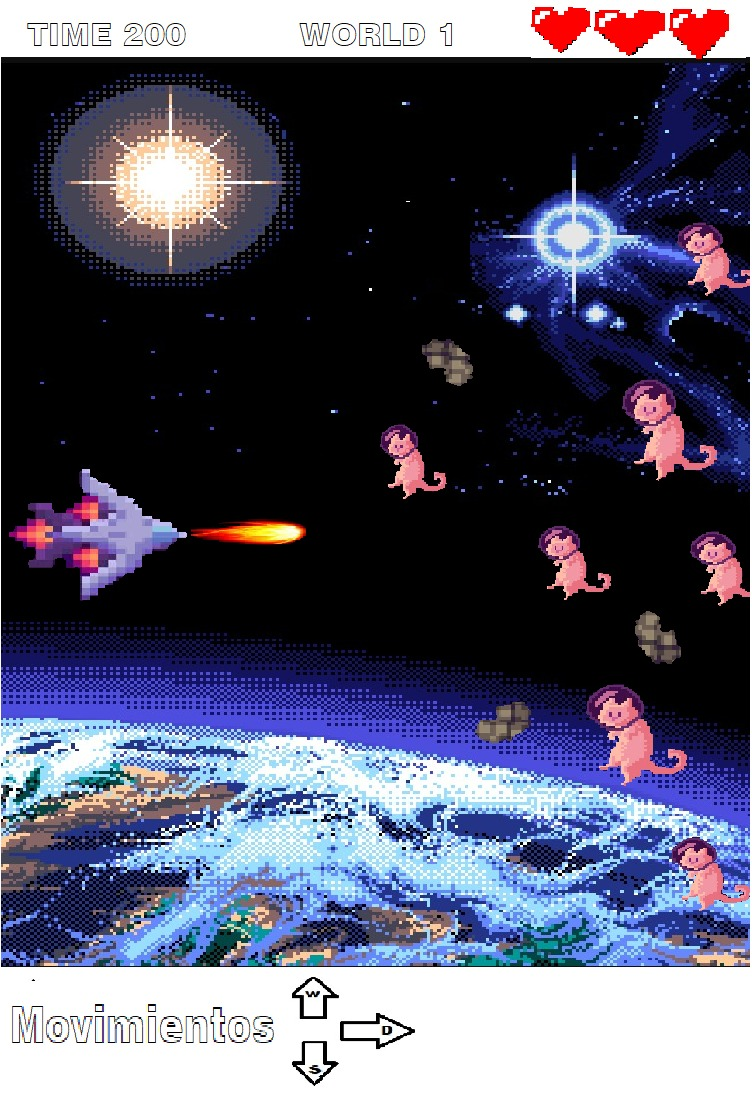
\includegraphics[scale=0.35]{Ideación/Images/movimientos.jpeg}


\subsection{Protagonistas}
Se contarán con ciertos personajes que se encuentran en búsqueda de ser los mejores exploradores intergalácticos, los cuales dispondrán de varias naves con tecnología cuántica capaz de sobrepasar las leyes de la física, que a su vez la diversidad de los niveles y mapas permitirán conocer nuevos confines galácticos con mayores dificultades. 

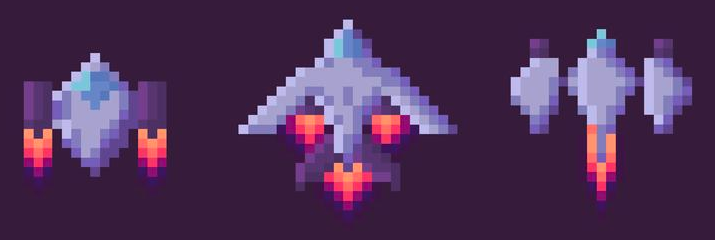
\includegraphics[scale=0.48]{Ideación/Images/protagonistas.png}

\subsubsection{Antagonistas}
Criaturas desconocidas que aumentan su poder y capacidad de ataque a medida que se avanza de nivel. Estos monstruos aparecerán de forma aleatoria a lo largo del juego, con el objetivo de interferir con la exploración de los personajes principales. Cabe anotar que, durante los diferentes niveles aparecerán diferentes personajes de la armada galáctica de saqueadores comandados por un jefe final conocido en el oscuro universo como "Galactic Burglar". 

Los personajes de la armada no efectuarán disparos hacia el personaje principal, sin embargo, si llega haber un contacto entre los protagonistas y los antagonistas se presenciará una supernova que destruirá tanto al protagonista como el antagonista y se terminara el juego. 

Por último, el jefe final podrá disparar bombas de energía a la velocidad de la luz que, si colisionan 5 veces con el personaje principal, lo destruirán inmediatamente. 

Enemigo 1: 



\includegraphics[scale=0.55]{Ideación/Images/enemigo.png}

Enemigo 2:


\includegraphics[scale=0.30]{Ideación/Images/enemigo2.png}

Jefe final: 



\subsection{Acciones}
Los jugadores se enfrentarán a la armada galáctica de saqueadores a los cuales se les podrá disparar rayos cósmicos. 
Los protagonistas podrán atacar con los poderes que irán apareciendo durante el mapa.

\subsection{Recursos}
A lo largo del juego se encontrarán meteoritos con dos posibles poderes escondidos en ellos que se le otorgaran al jugador, el primero es la capacidad de eliminar a todo el ejército de enemigos y pasar directamente a la fase de combate con el jefe final, el segundo es el de poder de atravesar por un agujero de gusano, tratándose de un atajo para alcanzar la meta y así subir de nivel. 
Para obtener el poder, el usuario deberá disparar y hacer explotar el meteorito.

\subsection{Eliminación}
El juego finaliza si los jugadores pierden todas sus vidas al ser atacados por los monstruos, o si no cumplen con el tiempo estipulado.

\subsection{Interacción}
Los jugadores podrán eliminar a las criaturas que irán emergiendo mientras se recorren las pistas galácticas.

\subsection{Modalidad}
El juego se diseñará para un solo jugador, quien podrá elegir distintas naves de carrera intergaláctica.

\subsection{Dificultad}
Mientras más avanza el jugador en las diferentes galaxias, más irá costando el ganar dentro de los diferentes mundos de acción, es decir, el nivel de dificultad aumentará pese tenga más recorrido y haya sobrepasado niveles inferiores. Además, las criaturas galácticas que aparecen en los niveles más altos, contarán con una tecnología más desarrollada, lo que implicará que esquivar sus ataques y/o destruirlos tomará más tiempo de lo habitual. 

\subsection{Finalidad}
Recolección de galaxias, planetas, estrellas, lo cual es necesario para convertirse en el mejor piloto intergaláctico de todo el universo conocible. 
\newpage

\bibliographystyle{IEEEtran}
\bibliography{references}
\cite{calistenia}


\end{document}
